\chapter{Exploratory data analysis}
Now that we have organized our dataset and have gained the nature of the features, we are ready to start examining the values of the features and response (target) feature. Understanding the effect of the values of the features on the decision of the customer to subscribe to a term-deposit or not is essential for a predictive Machine Learning model development. In the previous chapter we gained an understanding of our dataset by visualizing the frequency of customers the bank contacted during this telemarketing. However, our analysis in data wrangling did not reveal the effect of each feature value on the success of the telemarketing campaign. In this chapter we perform detailed analysis of feature values versus response (target) variable to reveal the importance of each feature as well as its unique value on the success rate of the telemarketing campaign. As in the previous chapter, we group the categorical and numerical features into related groups such as demographics, financial data, and campaign. 

\section{Subscription rate per job category}
The rate of customer subscription as well as the total number of subscribed customers per each job category is shown in figure \ref{fig:job_rate}. The figure shows that though the bank contacted the largest number of people in job segment category of blue-collar, and the number of students the bank contacted was the smallest, the percentage of students who subscribed to term deposit is the largest. We recommend the bank contact more students in the next telemarketing campaign.

\begin{figure}[tbh]
\centering
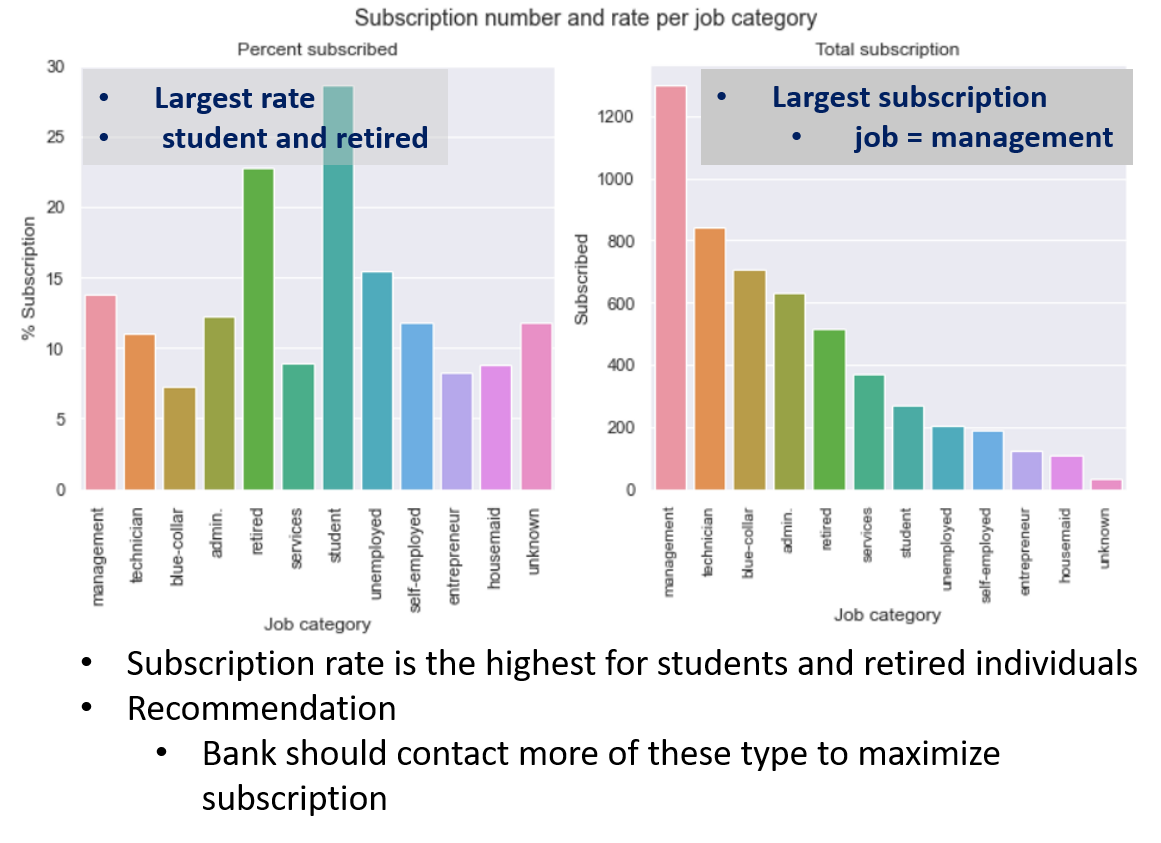
\includegraphics[width = 1.0\hsize]{./resources/img/fig_job_rate.png}
\caption{Rate of customer subscription and total subscribed number per job category} 
\label{fig:job_rate}
\end{figure}

\section{Subscription rate per marital status and educational level}
Customer subscription rate as well as the total number of subscribers per each marital status and educational level is shown in figure \ref{fig:marital_education_rate}
\begin{figure}[tbh]
\centering
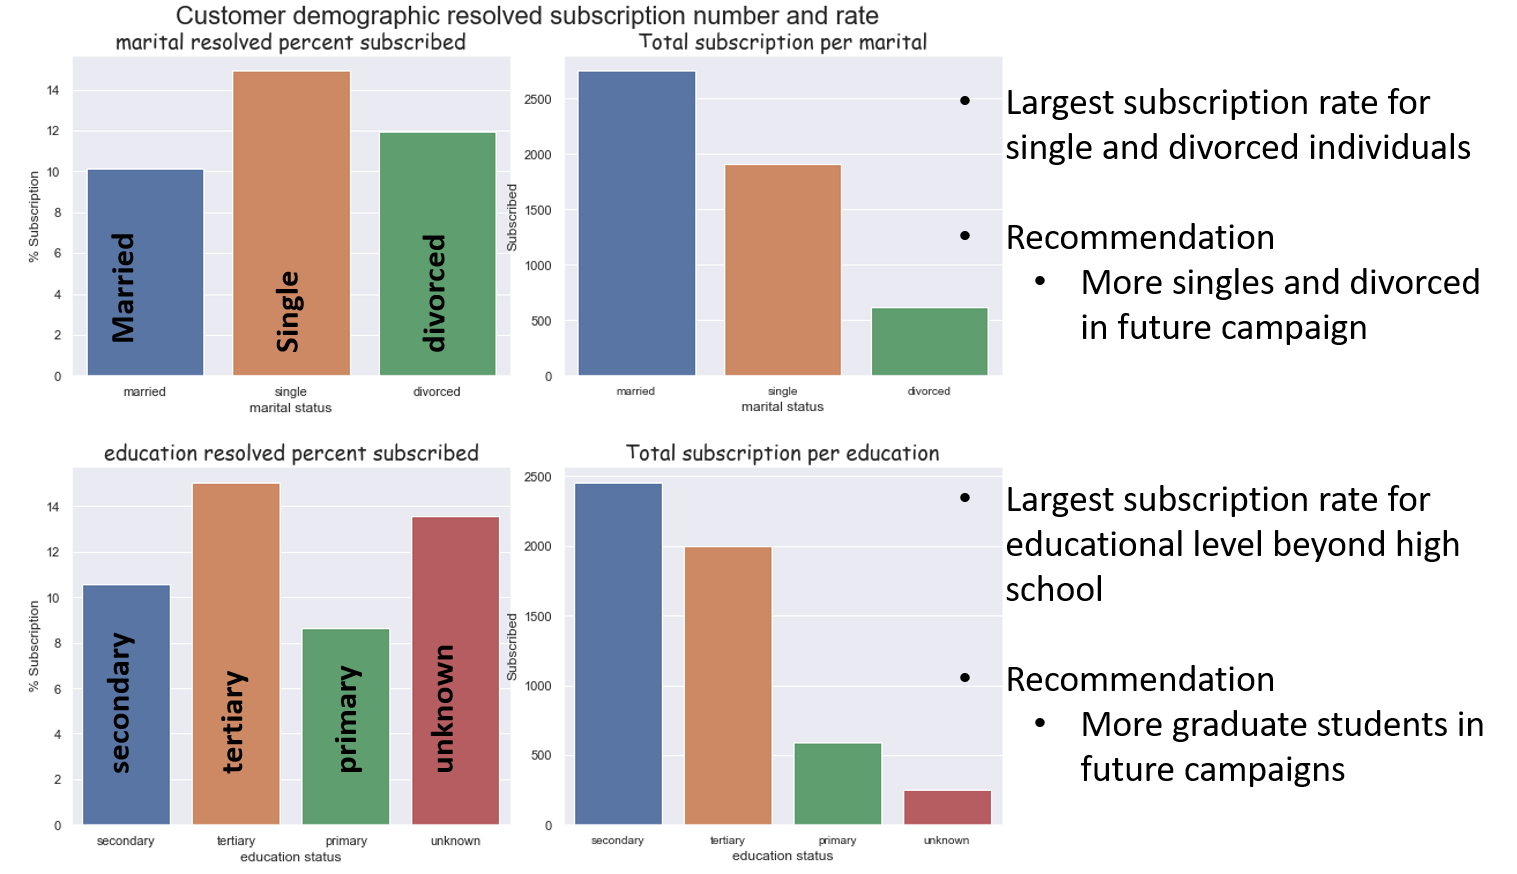
\includegraphics[width = 1.0\hsize]{./resources/img/fig_marital_education_rate.png}
\caption{Rate of customer subscription and total subscribed number per customer marital status and educational level.} 
\label{fig:marital_education_rate}
\end{figure}

\subsubsection*{Marital status}
The largest number of customers who subscribed are married. This is due to the bank contacted more married people during this telemarketing. Nevertheless, unmarried people are more likely to subscribe (50\% more probable than that of married people) though the total number of single subscribers is less than the total number of married subscribers. the rate of subscription for divorced people is also greater than that of married people. We recommend the bank target more single and divorced people in its next telemarketing campaign for term deposit subscription. In contrast, the most probable customers to enroll for the term deposit have completed tertiary level of education. The educational level of the second largest probable group to enroll for the term deposit is unknown; with subscription rate of approximately equal to the average of the three remaining groups. This corroborates the claim the telemarketer forgot to record the educational level of some of the customers contacted.

\subsubsection*{Educational level}
The largest number of subscribers have completed secondary education. Customers with unregistered unknown educational level are the least subscribers. The telemarketer might have forgotten to register or the customers might have not been willing to expose their educational level. In contrast, the most probable customers to enroll for the term deposit have completed tertiary level of education. The educational level of the second largest probable group to enroll for the term deposit is unknown; with subscription rate of approximately equal to the average of the three remaining groups. This corroborates the claim the telemarketer forgot to record the educational level of some of the customers contacted. Customers who completed primary education are the least subscribers and are least probable to subscriber. In its next telemarketing we recommend the bank target more customers who completed tertiary education.

\section{Subscription rate per customer financial segment}

Customer subscription rate as well as the total number of subscribers per customer's financial account is shown in figure \ref{} each marital status and educational level is shown in figure \ref{fig:marital_education_rate}
\begin{figure}[tbh]
\centering
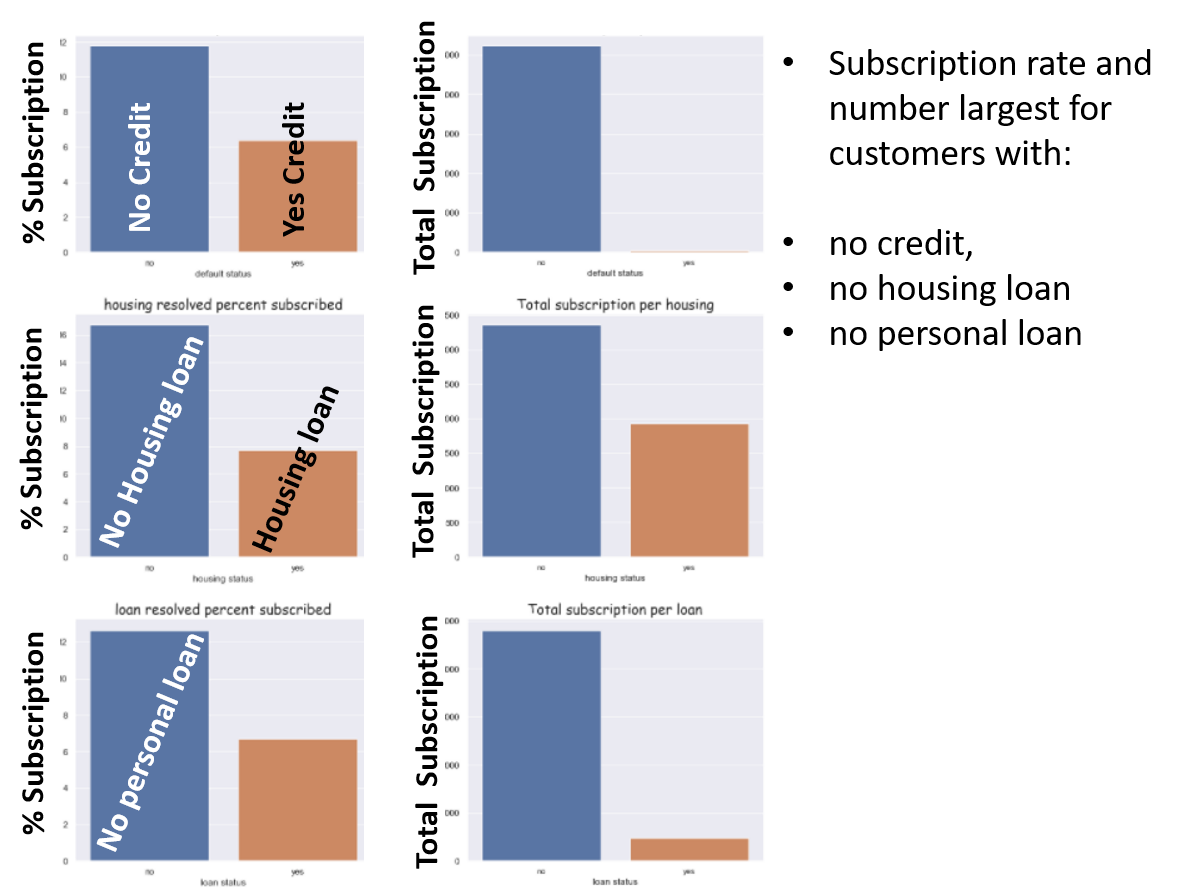
\includegraphics[width = 1.0\hsize]{./resources/img/fig_financial_rate.png}
\caption{Rate of customer subscription and total subscribed number per customer's status of financial account.} 
\label{fig:financial_rate}
\end{figure}

\subsubsection*{Credit}
The number of customers who have credit and subscribed to term deposit is negligibly small. Most subscribers do not have credit. Moreover, the subscription rate of customers with no credit is about 2 times higher than those with credit. In the next telemarketing, we recommend the bank focus on customers with no credit.

\subsubsection*{Housing loan}
The total number of subscribed customers as well as the rate of subscription is significantly higher for people with no housing loan as compared to customers that possess housing loan (about 2 times higher). This is consistent with our previous observation based on marital status of customers where the subscription rate is the highest for single (unmarried) people.

\subsubsection*{Personal loan}
Similarly, the number as well as rate of subscription is the largest for customer groups with no personal loans.

\section{Subscription rate per campaign details}
Customer subscription rate as well as the total number of subscribers per categories based on the details of the campaign such as the method of contact and the month the contact was conducted is shown in figure \ref{fig:campaign_rate}customer's financial account is shown in figure \ref{} each marital status and educational level is shown in figure \ref{fig:marital_education_rate}
\begin{figure}[tbh]
\centering
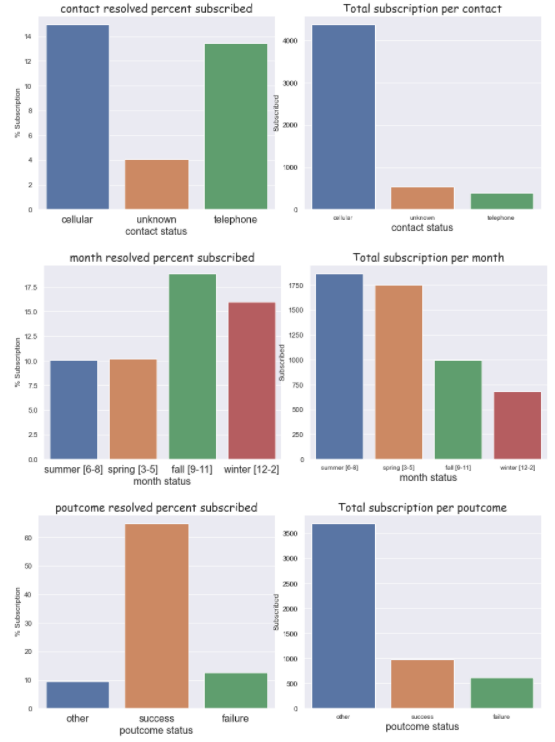
\includegraphics[width = 1.0\hsize]{./resources/img/fig_campaign_rate.png}
\caption{Rate of customer subscription and total subscribed number per details of campaign categories.} 
\label{fig:financial_rate}
\end{figure}

\subsubsection*{Method of contact}
Though the majority of the subscribed customers were enrolled throuth talling over cellular phones, the subscription rates for contacts with land line phones and cellular phones are comparable. The larger number of contacts and hence subscription via cellular phones could simply be due to the larger number of customers using cellular phones. Since, whether using cellular or land line does not yield to an appreciable change in subscription rate; the bank should not worry on the type of communication during its telemarketing. We will drop the feature contact during our machine learning developlment as it carries no significant impact on the targeting customers.

\subsubsection*{Contact season}
During this telemarketing the bank conducted the majority of its contacts during summer and spring seasons and obtained a large number of subscribers. Considering summer as a primary vacation season and spring the tax return season, the bank was able to contact a large number of people and get them subscribed. However, the subscription rate of the contacted customers is the highest during fall and winter season. Though this might be studies farther by including more historical data, during this campaign the bank would have better benefitted if it were to rigourously initiate its telemarketing during fall and winter seasons.

\subsubsection*{Previous outcome}
From the histogram plot of the previous outcome status of a customer as, we find that a customer who responded favourably during past campaign is more likely to respond favourably during the current campaign.

\section{Subscription rate per age group and balance group}
For ease of analysis, we have grouped the numerical features \hl{age, balance} into different practical groups. We grouped customers into groups of \hl{no balance, low balance, avg balance, and high balance} based on how high a customer's balance is compared to the average balance of the populations. Similarly, customers are also grouped into 4 different age groups with 15 years bin size. The subscription rate of customers versus age group and balance group is shown in figure \ref{fig:age_balance_rate}

\begin{figure}[tb]
\centering
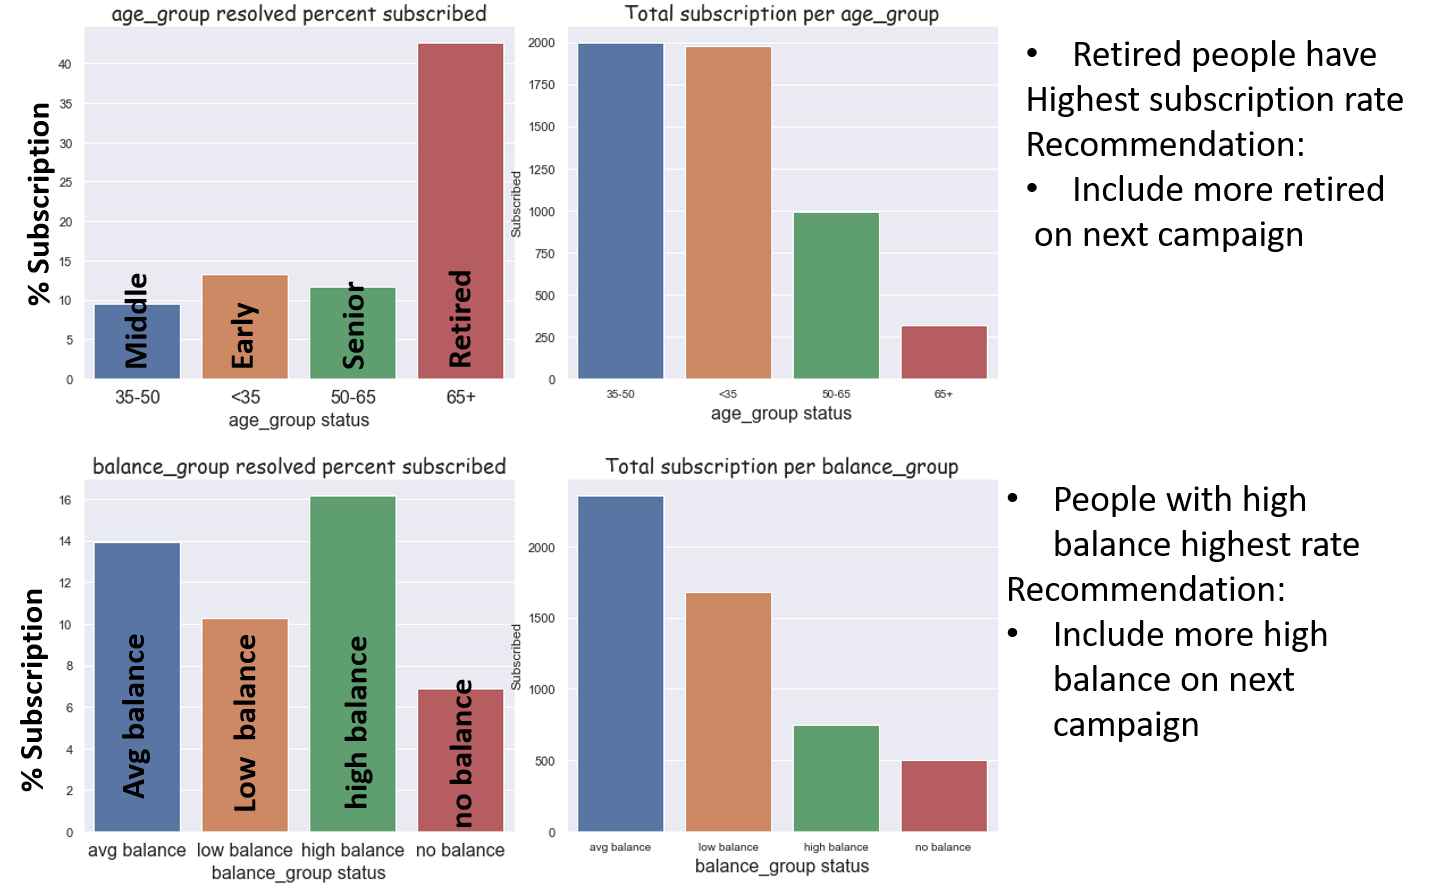
\includegraphics[width = 1.0\hsize]{./resources/img/fig_age_balance_rate.png}
\caption{Rate of customer subscription and total subscribed number per customer age group and customer balance level.} 
\label{fig:age_balance_rate}
\end{figure}



